%----------------------------------------------------------------------------------------
%	PACKAGES AND OTHER DOCUMENT CONFIGURATIONS
%----------------------------------------------------------------------------------------

\documentclass[12pt]{article}



\usepackage[utf8]{inputenc} % Required for inputting international characters

\usepackage[T1]{fontenc} % Output font encoding for international characters

\usepackage[top=2cm,right=2cm, left=2cm]{geometry} % set margins

\usepackage{setspace} % paragraph spacing

\usepackage{mathpazo} % Palatino font

\usepackage{hyperref}  % for hyperlinks to resources\

\usepackage{graphicx} % for logo


\usepackage{tcolorbox} % to color boxes


\usepackage{pgfgantt} % for gantt chart



\usepackage{tabularx} % in the preamble
\newcolumntype{Y}{>{\centering\arraybackslash}X}
\newcolumntype{b}{>{\hsize=.5\hsize}X} % column 1 = 50% of a column
\newcolumntype{s}{>{\hsize=.4\hsize}X} % column 2 = 40% of a column
\newcolumntype{m}{>{\hsize=1.1\hsize}X} % column 3 = 110% of a column

\definecolor{barblue}{RGB}{153,204,254}
\definecolor{groupblue}{RGB}{51,102,254}
\definecolor{linkred}{RGB}{165,0,33}
\renewcommand\sfdefault{phv}
%\renewcommand\mddefault{mc}
%\renewcommand\bfdefault{bc}
\setganttlinklabel{s-s}{START-TO-START}
\setganttlinklabel{f-s}{FINISH-TO-START}
\setganttlinklabel{f-f}{FINISH-TO-FINISH}

\renewcommand{\arraystretch}{2}

\begin{document}

%----------------------------------------------------------------------------------------
%	TITLE PAGE
%----------------------------------------------------------------------------------------

\begin{titlepage} % Suppresses displaying the page number on the title page and the subsequent page counts as page 1
	\newcommand{\HRule}{\rule{\linewidth}{0.5mm}} % Defines a new command for horizontal lines, change thickness here
	
	\center % Centre everything on the page
	
	%------------------------------------------------
	%	Headings
	%------------------------------------------------
	
	\textsc{\LARGE University of Regina}\\[1.5cm] % Main heading such as the name of your university/college
	
	\textsc{\Large ENSE 477: Capstone Project}\\[0.5cm] % Major heading such as course name
	
	\textsc{\large System and Object Design}\\[0.5cm] % Minor heading such as course title
	
	%------------------------------------------------
	%	Title
	%------------------------------------------------
	
	\HRule\\[0.4cm]
	
	{\huge\bfseries Telport: Sasktel Telecommunications Portal}\\[0.4cm] % Title of your document
	
	\HRule\\[1.5cm]
	
	%------------------------------------------------
	%	Author(s)
	%------------------------------------------------
	
	\begin{minipage}[t]{0.4\textwidth}
		\begin{flushleft}
			\large
			\textit{Authors}\\
			Dakota \textsc{Fisher}\\ % Your name
			200 344 336\newline \newline
			Quinn \textsc{Bast}\\ % Your name
			200 352 973
		\end{flushleft}
	\end{minipage}
	~
	\begin{minipage}[t]{0.4\textwidth}
		\begin{flushright}
			\large
			\textit{Supervisor}\\
			Dr. Yasser \textsc{Morgan} % Supervisor's name
		\end{flushright}
	\end{minipage}
	
	% If you don't want a supervisor, uncomment the two lines below and comment the code above
	%{\large\textit{Author}}\\
	%John \textsc{Smith} % Your name
	
	

%------------------------------------------------
	%	Logo
	%------------------------------------------------
		\vfill\vfill\vfill\vfill\vfill % Position the date 3/4 down the remaining page
	
\includegraphics[width=.5\textwidth]{UR_Logo_Primary_Full_Colour_RGB.jpg} % Include a department/university logo - this will require the graphicx package
	
	%------------------------------------------------
	%	Date
	%------------------------------------------------
	

	
	{Last Modified\\\large\today} % Date, change the \today to a set date if you want to be precise		

	
	 % Push the date up 1/4 of the remaining page
	 
	%----------------------------------------------------------------------------------------	
\end{titlepage}

%----------------------------------------------------------------------------------------


%----------------------------------------------------------------------------------------
% Revision History
%----------------------------------------------------------------------------------------
\section*{Revision History}
\begin{tabularx}{\textwidth}{|Y|Y|Y|}
\hline
  \textbf{Revision Version} & \textbf{Revision Author} & \textbf{Revision Date}\\
\hline
1.0 & Quinn Bast & February 23, 2019 \\
\hline
\end{tabularx}

\newpage


%----------------------------------------------------------------------------------------
%	Table of Contents
%----------------------------------------------------------------------------------------

\pagestyle{plain} %get rid of header/footer for toc page
\pagenumbering{roman}

\tableofcontents %put Table of Contents in
\cleardoublepage %start new page

\listoffigures %put List of Figures in
\cleardoublepage %start new page

\listoftables %put List of Tables in
\cleardoublepage %start new page

\pagestyle{plain} % put headers/footers back on
\pagenumbering{arabic}

%----------------------------------------------------------------------------------------

%----------------------------------------------------------------------------------------
%	Body of Document
%----------------------------------------------------------------------------------------
%----------------------------------------------------------------------------------------
\doublespacing % set document to be default double spaced

%----------------------------------------------------------------------------------------
%	Problem Statement
%----------------------------------------------------------------------------------------
\section{Problem Statement}
\paragraph{} 
	SaskTel requires a communications portal that can interwork with a Telephony Application Server and our core network to present communications and feature capabilities through a browser.  This will allow for the exploration of new communications service models. 
\paragraph{} 
	SaskTel has been pursuing the deployment of a new communications core along with the Cisco/Broadsoft Telephony Application Server branded as Broadworks.  One of the drivers is to enable a richer customer experience through a converged architecture that exposes rapid development to enables new capabilities.  Broadworks exposes the Application Programming Interface to access service control tools and user information.  These tools and information can be used to create new communications applications or add additional value to existing applications.  
\paragraph{} 
	The main objectives for SaskTel is to gain exposure to new and innovative communications service experience for our customers and to promote the potential internally for aligning resources, time and effort in enabling applications.
\pagebreak

%----------------------------------------------------------------------------------------
%	System Architecture
%----------------------------------------------------------------------------------------
\section{System Architecture}
\paragraph{}
	The application that is being created is a web server which will enable customer to configure various settings about their account's calling settings. This will enable customers to be able to seamlessly change their phone's settings without the need to contact any support lines. Furthermore, SaskTel has realized the need to convert their services to the world wide web. Customers are moving away from home phones because of the development of mobile technologies. Accessibility to your phone no matter where you are is becoming a necessity for customers. Thus, SaskTel has the need to be able to make phone calls from the internet browser. This requires interfacing with SaskTel's WebRTC gateway in order to make communications possible between a web browser and a mobile device.
	
	
\paragraph{}
	SaskTel has a large infrastructure already established and thus, have many of the required components for this project already in place, the missing components are the client-facing components of the application. The main components are the IMS core, Home Subscriber System (User Profile Repository), Telephony Application Server, WebRTC Gateway, gateway access to the PSTN, and SIP clients. These network components will interface with our architecture as shown in the image below.

	\begin{figure}
	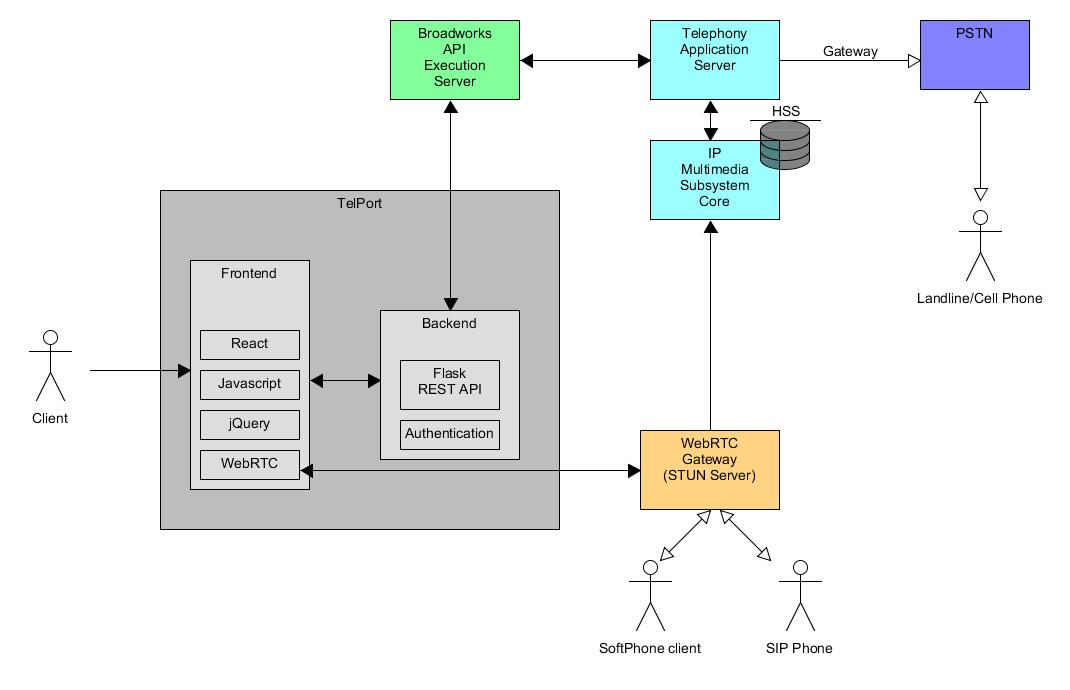
\includegraphics[width=\textwidth]{ServerArchitecture.jpg}
	\caption{TelPort Network Architecture}
	\end{figure}

\pagebreak
\subsection{Major SaskTel Components}
\subsubsection{BroadWorks API Execution Server}
\paragraph{}
	BroadWorks VoIP communications application server enables service providers to offer a comprehensive portfolio of business and consumer communications applications and value added applications from a common network platform. BroadWorks delivers communication solutions that integrate video, fax, voice and email communications for businesses and consumers worldwide whether through IP PBX/Centrex, Mobile PBX, Business Line, Trunking and consumer solutions.  BroadWorks goes beyond connecting an IP pipe to a user. The advanced calling features allow service providers the ability to offer innovative, compelling, revenue-generating solutions to both business and residential customers.
 
\paragraph{}
	The BroadWorks Application Server operates at the core of BroadWorks and is responsible for the execution of all enhanced personal and group features. The server's database maintains user and group profiles, as well as service and subscription data. The Application Server supports a variety of access side protocols in including SIP and MGCP.
 
 \paragraph{}
	In addition to the self-care web portal and a variety of desktop client applications, BroadWorks provides a very rich set of open programmable interfaces called the Xtended Services Interface (Xsi) that allows operators, partners and even end users to build their own niche applications around the services offered by BroadWorks.  The Xsi is a RESTful HTTP based interface that uses simple commands to enable service configuration, click to dial and other call control primitives over the web. TheBroadSoft Xtended program gives operators access to a growing community of software developers that have adopted the Xsi and are building innovative applications and web mashups based on the BroadWorks platform.

\subsubsection{IP Multimedia Subsystem}
\paragraph{}
	IMS (IP Multimedia Subsystem – architectural framework) provides control functions within the Telecom network core, allowing for shared use of infrastructure and services across fixed and mobile technologies.  IMS provides a path to transition the core of a telecom network to IP.  IMS will be used in the Demo to facilitate subscriber registration onto the network, allow the use of directory numbers to address and direct calls and to provide a bridge between the internet and the legacy PSTN.

\paragraph{}
	SaskTel is pursuing the installation of IMS as a foundation to provide broader services, converged services (fixed and mobile), and to generate service differentiators to maintain a competitive edge.  SaskTel will strive to align the majority of communications services to be delivered from a single (geo-redundant) core.  As solutions evolve, it is expected that the core IMS functions will reside on common computing hardware.  SaskTel will leverage IMS to function as a bridge between legacy communications and communications on the internet, thus migrating the PSTN to the internet.

\subsubsection{WebRTC Gateway}
\paragraph{}
	Within SaskTel's environment, a WebRTC Gateway will be added to provide an interface between the use of web centric protocols and Telecom IP network protocols.  Simply stated, the WebRTC gateway gives the ability for a service on a browser to communicate with IMS.  This allows the bridging between WebRTC on the Web and IMS subscription, IMS service and access to the PSTN.  By using this interconnection, a user can be identified with a Phone number, access a network address book and place calls between the web and the PSTN.  

\subsubsection{Home Subscriber System}
\paragraph{}
	The Home Subscriber System (HSS) is accessed by the IMS Core in order to obtain information about a user. This is how the BroadWorks API accesses information about the various users and this is also how our application is able to access user information without the need of a database. Because everything is stored externally, our application never needs to store any information about a user.
	
\subsection{Major TelPort Components}
\subsubsection{Flask REST API}
\paragraph{}
	Without our application, the frontend can communicate directly with the BroadWorks API, however, in order to do so, the frontend needs to keep track of a user's login tokens. This exposes the user's tokens and credentials to the frontend in an unsafe manner which is vulnerable to XSS (Cross-site scripting) attacks. As a result, our application makes use of an additional layer of security through our backend before being able to contact the Broadsoft server.
	
\paragraph{}
	The REST API for our backend is very small, containing only 4 endpoints. The endpoints provided by our backend server are described in detail as follows:
	
	\begin{tcolorbox}
	POST	/rest/login
	\end{tcolorbox}
	\paragraph{}
		\textbf{Description:} Allows the user to login to the application.
		
\paragraph{}
		\textbf{Request Body:}
	
		%------------------------------------------------------------
		% 	POST  /rest/login
		%------------------------------------------------------------
		\begin{table}[htb]
		\centering
		\begin{tabularx}{\textwidth}{|s|s|m|m|}
		\hline
			\textbf{Parameter} & \textbf{Type} & \textbf{Description} & \textbf{Example} \\
		\hline
			username & 
			String & 
			The user's username to login with. & 
			SampleUser123 \\
		\hline
			password & 
			String & 
			The user's password. & 
			hunter123 \\
		\hline
		\end{tabularx}
		\end{table}
		
	\begin{tcolorbox}
	POST /rest/logout
	\end{tcolorbox}
	
\paragraph{}
		\textbf{Description:} Logs the user out of the application. NOTE: Requires a valid token.
\paragraph{}
		\textbf{Request Body:} None \\
		
	
\paragraph{}
	\begin{tcolorbox}
	POST /rest/token/refresh
	\end{tcolorbox}
	
\paragraph{}
		\textbf{Description:} Refreshes the user's session token to further their login session. This is automatically requested by the frontend when needed. NOTE: Requires a valid token.
		
\paragraph{}
		\textbf{Request Body:} None \\
		
\paragraph{}
	
	\begin{tcolorbox}
	POST /rest/broadsoft
	\end{tcolorbox}
\paragraph{}
	\textbf{Description:} Accesses the BroadWorks API Execution server. NOTE: Requires a valid token.
\paragraph{}
	\textbf{Request Body:}
			%------------------------------------------------------------
		% 	POST  /rest/broadsoft
		%------------------------------------------------------------
		\begin{table}[htb]
		\centering
		\begin{tabularx}{\textwidth}{|s|s|m|m|}
		\hline
			\textbf{Parameter} & \textbf{Type} & \textbf{Description} & \textbf{Example} \\
		\hline
			endpoint & 
			String & 
			A BroadWorks REST API endpoint to access & 
			/user/<user>/services \\
		\hline
			method & 
			String & 
			The method to access the BroadWorks REST API endpoint through. & 
			"PUT", "GET", "POST", etc... \\
		\hline
			data & 
			Xml String & 
			An XML formatted string to send to the BroadWorks API. The data to send is as defined int he BroadWorks API. & 
			<?xml version="1.0" encoding="ISO-8859-1"?>
			<DoNotDisturb>
		    <active> false </active>
		    <ringSplash> false </ringSplash>
			</DoNotDisturb> \\
		\hline
		\end{tabularx}
		\end{table}
	
	\pagebreak
\subsubsection{WebRTC}
\paragraph{}
	In order to enable the capability to make calls from the web, WebRTC is required for our web application to interface with an SIP client. There is quite a bit of overhead to convert a WebRTC session to an SIP session, however. Therefore, the use of a JavaScript library JsSIP was used in order to help make this process easier. The use of this framework requires some basic server configurations that were provided from SaskTel. Once this information was obtained, making calls from the web browser was quite simple to perform.

\pagebreak
	
\section{Class Diagrams}
\subsection{Backend Class Diagram}


	\begin{figure}[htb]
	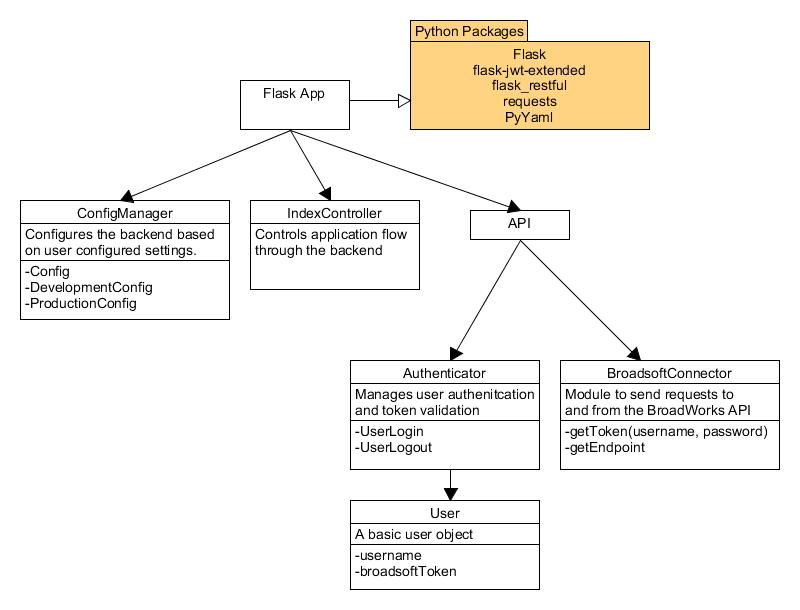
\includegraphics[width=\textwidth]{BackendClassDiagram.jpg}
	\caption{Backend Class Diagram}
	\end{figure}
	
	\pagebreak

\subsection{Frontend Class Diagram}
	
	\begin{figure}[htb]
	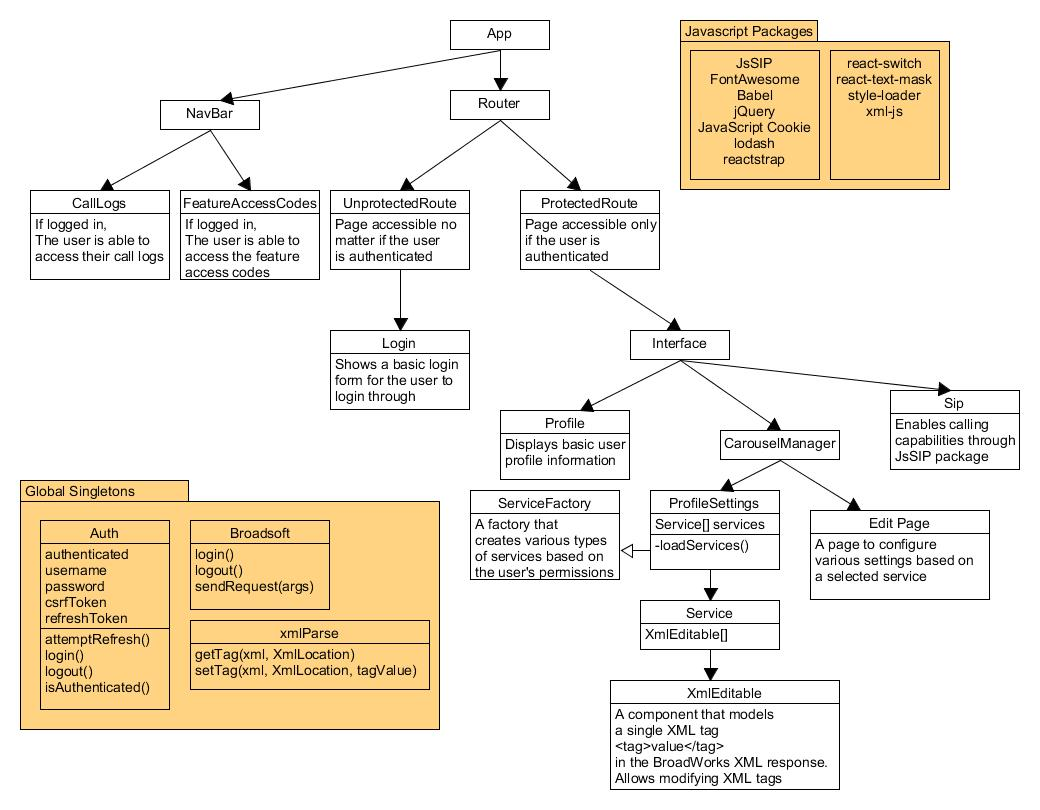
\includegraphics[width=\textwidth]{FrontendClassDiagram.jpg}
	\caption{Frontend Class Diagram}
	\end{figure}


%----------------------------------------------------------------------------------------
%	Frameworks, Libraries, and other tools
%----------------------------------------------------------------------------------------
\pagebreak
\section{Frameworks, Libraries, and other tools}

\subsection{Backend python packages}
\subsubsection{Flask JWT Extended}
\paragraph{}
	\href{https://flask-jwt-extended.readthedocs.io/en/latest/}{Flask-JWT-Extended} is a python library that adds support for using JSON Web Tokens (JWT) to Flask for protecting views. This allows our application to send information to the frontend while also only allowing authorized users to access the server. Additionally, Flask JWT Extended provides many helpful features built in to make working with JSON Web Tokens easier and more secure. This includes creating tokens from complex objects or complex object from received tokens, creating refresh tokens, token freshness and separate view decorators to only allow fresh tokens, token revoking/blacklisting, storing tokens in cookies and CSRF protection.


\subsubsection{Flask Restful}	
\paragraph{}
	\href{https://flask-restful.readthedocs.io/en/latest/}{Flask-RESTful} is an extension for Flask that adds support for quickly building REST APIs. Flask Restful makes creating REST endpoints and server responses extremely easy. Flask Restful requires minimal setup and only requires you to define the URL's for each REST endpoint and what function/class methods correspond to the endpoint. Flask Restful is extremely lightweight but extremely powerful.
	
\subsubsection{Requests}	
\paragraph{}
	\href{http://docs.python-requests.org/en/master/}{Requests} is a python library for sending HTTP requests from a server. Because our backend needs to interface with the BroadWorks API Execution server, using the Requests library is required for our application in order to talk to the BroadWorks API. Compared to the built-in python http library, Requests is significantly easier to use. Because of this, using this library saves a significant amount time and headache compared to using the default library.
	
\subsubsection{PyYaml}	
\paragraph{}
	Flask uses Yaml configuration files in order to setup some of its components. Because we wanted to allow our Flask application to output logs from the server, we needed to customize the Flask logging system which requires a Yaml configuration file. Using \href{https://pyyaml.org/wiki/PyYAMLDocumentation}{PyYaml} allows python to read the Yaml file and turn it into a python object that is able to be easily parsed by Flask.

\subsection{Frontend Javascript libraries}
\subsubsection{JsSIP}	
\paragraph{}
	WebRTC allows communication across two different browsers through the user of web sockets. In order to create a call from our web application, the client needs to be using a WebRTC connection, however, the RTC connection needs to be converted into the SIP protocol in order to communicate with a user's cellular device. Converting between RTC and SIP protocols is a complicated task, luckily, \href{https://jssip.net/}{JsSIP} does it automatically. By simply configuring the SIP settings, creating a call from the web is extremely easy with the use of this framework.
	
\subsubsection{FontAwesome}	
\paragraph{}
	\href{https://fontawesome.com/}{Font Awesome} is a collection of vector icons and logos that are free to use for the web. The use of icons within a web application lets a user more easily understand what a button or action will do based on the icon that is provided. This provides consistency between websites and also makes using the application easier for the user as they can simply recognize the icons that perform specific actions instead of having to search around.
	
\subsubsection{Javascript Cookie}	
\paragraph{}
	\href{https://github.com/js-cookie/js-cookie}{Javascript Cookie} allows Javascript code to access the browser's cookies. Because of the use of Flask JWT Extended in the backend, CSRF tokens are sent in cookies to the browser. Accessing the cookies from the browser is possible, but somewhat complicated. Javascript Cookie makes accessing browser cookies much easier, and allows future Ajax requests to be configured with the cookies that have been sent from the backend to validate the user.
	
\subsubsection{ReactStrap}	
\paragraph{}
	\href{https://reactstrap.github.io/}{Reactstrap} is a javascript package to allow the use of Bootstrap 4 components within React. Bootstrap makes styling a website extremely, taking time away from styling CSS sheets to get the website how you want it to look. By using boostrap, only minor CSS changes need to be made while the default components will position elements in the website with minimal configurations.
	
	
\subsubsection{React Switch}	
\paragraph{}
	Toggle buttons and sliders are not a default element in HTML5 and are not an included element in bootstrap. However, in our application, toggling various settings between "On" and "Off" is a large part of the application. Toggle buttons are the easiest way to indicate if something is on or off. \href{https://www.npmjs.com/package/react-switch}{React Switch} provides the ability to put a toggle buttons on a react page. This allows us to easily show if a setting is on or off.
	
\subsubsection{React Text Mask}	
\paragraph{}
	When a user types into a textbox, their input is unreliable. They might make a typo or format the text improperly. This is where \href{https://www.npmjs.com/package/react-text-mask}{React Text Mask} is extremely useful. Typing a phone number might require an area code, or it might require a "+1" at the front. In order to eliminate any confusion for the user, React Text Mask allows us to specify a mask: (\_\_\_)\_\_\_-\_\_\_\_ and this mask guides the user's input. The user cannot break elements from the mask, ensuring that their input is properly formatted. The users are forced to input a specific character set which is verified based on a RegEx. This allows us to ensure that a user is inputting the correct information and takes any confusion away the users because they know the information they are entering is correct. Of course, this does not replace backend security and validation, but simply provides end users with a better experience.
	
\subsubsection{Xml-js}	
\paragraph{}
	\href{https://www.npmjs.com/package/xml-js}{Xml-js} allows converting XML into Javascript or JSON objects. Because the BroadWorks API sends an XML response, we need to be able to parse, read, and modify XML. This library allows parsing XML objects in order to read values to display to the user, and modify values to send back to the BroadWorks API. This package is a necessity for our application as 80\% of the application needs to examine XML data.
	
\subsection{Other tools}
\paragraph{}	The following sections denote tools that are utilized or were considered to be of use during the project's development. Programs and tools, alongside their effective alternatives are discussed to get an understanding of what, and why tools were picked or not picked to be used to benefit the work flow of the project. Every reference to an application in the following sections has a direct hyperlink reference if clicked on using an electronic medium.

\subsubsection{\href{https://Github.com}{Github}}
\paragraph{}	Git is a powerful source version control solution that allows for multiple developers to collaborate on  a project. The Git provider used during this project is \href{https://Github.com}{Github}. Not only does it allow for collaborative features, it also allows for parallel streams of development of many features. The tool also allows for public display of the project, to allow for open source development if the repository is not kept private. A key feature and benefit of using Git is that it allows for projects to commit checkpoints and milestones in development, such that if an update isn't beneficial, it can easily be reverted to a previously confirmed viable version.

\subsubsection{\href{https://toggl.com}{Toggl}}
\paragraph{}	\href{https://toggl.com}{Toggl} is a time tracking web application that allows teams to track their hours along with the project, and tags that correspond to the work that they are doing. This allows for us to track documentation time seperate from programming time and research time. While still keeping a total cumulative track of our time spent on the project. Ideally, the time tracking entries are relative to our commits on \href{https://Github.com}{Github}. Of the options online at the time, this is the only option that we felt met the requirements we needed to easily and painlessly manage our project time.

\subsubsection{\href{https://www.gitkraken.com/}{GitKraken}}
\paragraph{}	The tool \href{https://www.gitkraken.com/}{GitKraken} is a powerful Git version control client that has an easily manageable interface. It also has the ability to see how each branch correlates to one another, and resolve any conflicts within the application directly. There isn't any particular reason to use this tool over another alternative such as \href{https://desktop.github.com/}{GitHub Desktop}, \href{https://www.sourcetreeapp.com/}{SourceTree}, or \href{https://gitforwindows.org/}{GitBash}, but it definitely was a nice discovery for our quality of life work flow. 

\paragraph{} The company that created GitKraken, also has a product called \href{https://www.gitkraken.com/glo}{Glo Boards}. The application is functionally equivalent to \href{https://trello.com/en}{Trello}. Both programs allow for a team to manage issues on a \href{https://github.com}{GitHub} repository easily and visualize changes into KanBan board styles. The decision to use a KanBan board software instead of just the issue tracking software on \href{https://github.com}{GitHub} was because it provides additional work flow improvements while still allowing \href{https://github.com}{GitHub} issues to still work normally.

\subsubsection{\href{https://drive.google.com}{Google Drive}}
\paragraph{}	For file containment and collaborative efforts, \href{https://drive.google.com}{Google Drive} was utilized to create rough drafts and documentation. The documents on \href{https://drive.google.com}{Google Drive} are deliberately kept out of the project as they provide no benefit and are unpolished in comparison to the products that should be present in the project. As files become absolute, and documentation gets refined and compiled into information that has enough value to be displayed, it is transferred to \href{https://github.com}{GitHub} to be displayed alongside other documentation. Other alternative data solutions that could have been used involve \href{https://onedrive.live.com/}{OneDrive} and \href{https://dropbox.com}{DropBox}, but the simultaneous access and collaborative nature of the \href{https://drive.google.com}{Google Drive} made it an ideal environment for rough collaborative drafting. 

\subsubsection{Discord}
\paragraph{}
	Being able to communicate with each other during the project is essential for collaboration. \href{https://discordapp.com/}{Discord} allows us to keep each other up to date on our day-to-day progress and ensures that we can both stay in contact throughout the creation of the project. \href{https://discordapp.com/}{Discord} provides a significant amount of functionality to enable functionality. This main functionality of discord is its text and voice chat capabilities. Keeping each other up to date is easy through text chat and allows us to send quick ideas back and forth while developing the project. Furthermore, voice chat allows us to communicate more vital information at a faster speed. While in a voice chat, \href{https://discordapp.com/}{Discord} provides the ability to share screens between users, making discord extremely useful for paired programming sessions and bug fixing.

	

\end{document}

%----------------------------------------------------------------------------------------
%	Document Style Templates
%----------------------------------------------------------------------------------------
%%%%%%%%%%%%%%%%%%%%%%%%%%%%%%%%%%%%%%%%%
% Section Nesting for Table of Contents
%
% A section or subsection can contain any number of nested children
%
%%%%%%%%%%%%%%%%%%%%%%%%%%%%%%%%%%%%%%%%%
% \section{First Title} %x
% \paragraph{} **~ Contents of First Title ~**
%
% \subsection{Second Title} %x.x
% \paragraph{} **~ Contents of Second Title ~**
%
% \subsubsection{Third Title} %x.x.x
% \paragraph{} **~ Contents of Third Title ~**
% 
% No more nesting allowed. capped at x.x.x sectioning
%
%
%%%%%%%%%%%%%%%%%%%%%%%%%%%%%%%%%%%%%%%%%
%
%----------------------------------------------------------------------------------------

%----------------------------------------------------------------------------------------
%	Template References and Licenses
%----------------------------------------------------------------------------------------
% This paper integrates the following templates into a single document.
% There is no endorsement in any way shape or form from the template authors.
%
%%%%%%%%%%%%%%%%%%%%%%%%%%%%%%%%%%%%%%%%%
% Academic Title Page
% LaTeX Template
% Version 2.0 (17/7/17)
%
% This template was downloaded from:
% http://www.LaTeXTemplates.com
%
% Original author:
% WikiBooks (LaTeX - Title Creation) with modifications by:
% Vel (vel@latextemplates.com)
%
% License:
% CC BY-NC-SA 3.0 (http://creativecommons.org/licenses/by-nc-sa/3.0/)
% 
%
%%%%%%%%%%%%%%%%%%%%%%%%%%%%%%%%%%%%%%%%%
